\documentclass[tikz, border = 1 cm]{standalone}

%%%%%%%%%%%%%%
\usepackage{tikz}
\usepackage{pgfplots}
\usetikzlibrary{positioning}
\usetikzlibrary{arrows}

\definecolor{blue1}{RGB}{0,177,234}
\definecolor{blue4}{RGB}{178,231,248}
\definecolor{gray1}{RGB}{76,84,93}
\definecolor{gray2}{RGB}{129,135,141}	
\definecolor{gray4}{RGB}{201,203,206}
%%%%%%%%%%%%%%

%%%%%%%%%%%%%%
%%%%%%%%%%%%%%
%%%%%%%%%%%%%%
\begin{document}

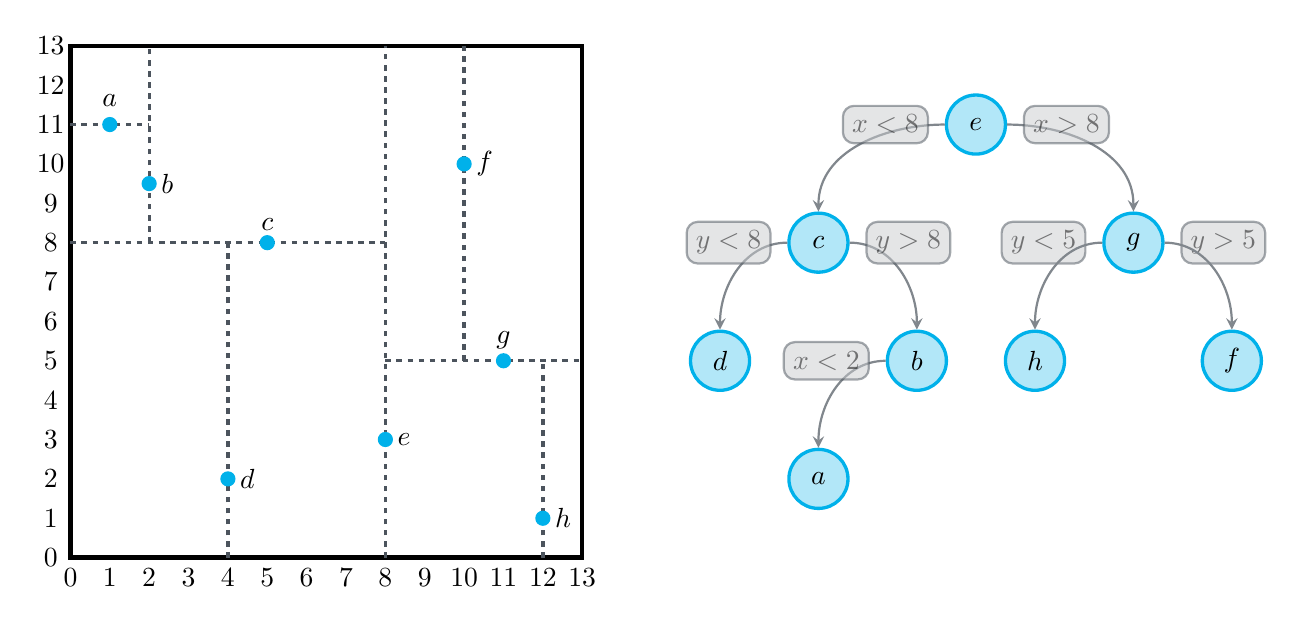
\begin{tikzpicture}[	scale=0.5, node distance=0.03cm,
				nosep/.style={inner sep=0pt, outer sep=0pt},
				pt/.style={scale=0.5, circle, minimum size=0.3cm, fill=blue1, draw=blue1, very thick, nosep},
				line/.style={draw=gray1, very thick, dash pattern=on 2pt},
				grnode/.style={circle, minimum size=0.75cm, fill=blue4, draw=blue1, very thick},
				box/.style={rectangle, thick, draw=gray1, fill=gray4, opacity=0.5, rounded corners},
				arrow/.style={thick, gray2, -stealth}
				]

	\draw[ultra thick, black] (0,0)--(13,0)--(13,13)--(0,13)--cycle ;
	\foreach \x in {0,...,13}
		\node at (\x,-0.5) {\x};
	\foreach \x in {0,...,13}
		\node at (-0.5,\x) {\x};

	\draw[line] (0,11) -- (2,11);
	\draw[line] (2,8) -- (2,13);
	\draw[line] (0,8) -- (8,8);
	\draw[line] (4,0) -- (4,8);
	\draw[line] (8,0) -- (8,13);
	\draw[line] (8,5) -- (13,5);
	\draw[line] (10,5) -- (10,13);
	\draw[line] (12,0) -- (12,5);
	
	\node[pt] (a) at (1,11) {};
	\node[pt] (b) at (2,9.5) {};
	\node[pt] (c) at (5,8) {};
	\node[pt] (d) at (4,2) {};
	\node[pt] (e) at (8,3) {};
	\node[pt] (f) at (10,10) {};
	\node[pt] (g) at (11,5) {};
	\node[pt] (h) at (12,1) {};
	
	\node[above=of a] (ta) {$a$};
	\node[right=of b] (tb) at (2,9.5) {$b$};
	\node[above=of c] (tc) at (5,8) {$c$};
	\node[right=of d] (td) at (4,2) {$d$};
	\node[right=of e] (te) at (8,3) {$e$};
	\node[right=of f] (tf) at (10,10) {$f$};
	\node[above=of g] (tg) at (11,5) {$g$};
	\node[right=of h] (th) at (12,1) {$h$};
	
	\tikzset{shift={(23,11)}}
	
	\node[grnode] (ne) at (0,0) {$e$};
	
	\node[grnode] (nc) at (-4,-3) {$c$};
	\node[grnode] (ng) at ( 4,-3) {$g$};
	
	\node[grnode] (nd) at (-6.5,-6) {$d$};
	\node[grnode] (nb) at (-1.5,-6) {$b$};
	\node[grnode] (nh) at (1.5,-6) {$h$};
	\node[grnode] (nf) at (6.5,-6) {$f$};
	
	\node[grnode] (na) at (-4,-9) {$a$};
	
	\draw[arrow] (ne.west) to[out=180,in=90] (nc.north);
	\node[box,left=0.2cm of ne] {$x<8$};
	\draw[arrow] (ne.east) to[out=0,in=90] (ng.north);
	\node[box,right=0.2cm of ne] {$x>8$};
	\draw[arrow] (nc.west) to[out=180,in=90] (nd.north);
	\node[box,left=0.2cm of nc] {$y<8$};
	\draw[arrow] (nc.east) to[out=0,in=90] (nb.north);
	\node[box,right=0.2cm of nc] {$y>8$};
	\draw[arrow] (nb.west) to[out=180,in=90] (na.north);
	\node[box,left=0.2cm of ng] {$y<5$};
	\draw[arrow] (ng.west) to[out=180,in=90] (nh.north);
	\node[box,right=0.2cm of ng] {$y>5$};
	\draw[arrow] (ng.east) to[out=0,in=90] (nf.north);
	\node[box,left=0.2cm of nb] {$x<2$};

\end{tikzpicture}
%%%%%%%%%%%%

\end{document}